% Created 2023-08-10 to 09:18
% Intended LaTeX compiler: pdflatex
\documentclass[12pt]{article}

%%%% settings when exporting code %%%% 

\usepackage{listings}
\lstdefinestyle{code-small}{
backgroundcolor=\color{white}, % background color for the code block
basicstyle=\ttfamily\small, % font used to display the code
commentstyle=\color[rgb]{0.5,0,0.5}, % color used to display comments in the code
keywordstyle=\color{black}, % color used to highlight certain words in the code
numberstyle=\ttfamily\tiny\color{gray}, % color used to display the line numbers
rulecolor=\color{black}, % color of the frame
stringstyle=\color[rgb]{0,.5,0},  % color used to display strings in the code
breakatwhitespace=false, % sets if automatic breaks should only happen at whitespace
breaklines=true, % sets automatic line breaking
columns=fullflexible,
frame=single, % adds a frame around the code (non,leftline,topline,bottomline,lines,single,shadowbox)
keepspaces=true, % % keeps spaces in text, useful for keeping indentation of code
literate={~}{$\sim$}{1}, % symbol properly display via latex
numbers=none, % where to put the line-numbers; possible values are (none, left, right)
numbersep=10pt, % how far the line-numbers are from the code
showspaces=false,
showstringspaces=false,
stepnumber=1, % the step between two line-numbers. If it's 1, each line will be numbered
tabsize=1,
xleftmargin=0cm,
emph={anova,apply,class,coef,colnames,colNames,colSums,dim,dcast,for,ggplot,head,if,ifelse,is.na,lapply,list.files,library,logLik,melt,plot,require,rowSums,sapply,setcolorder,setkey,str,summary,tapply},
aboveskip = \medskipamount, % define the space above displayed listings.
belowskip = \medskipamount, % define the space above displayed listings.
lineskip = 0pt} % specifies additional space between lines in listings
\lstset{style=code-small}
%%%% packages %%%%%

\usepackage[utf8]{inputenc}
\usepackage[T1]{fontenc}
\usepackage{lmodern}
\usepackage{textcomp}
\usepackage{color}
\usepackage{graphicx}
\usepackage{grffile}
\usepackage{wrapfig}
\usepackage{rotating}
\usepackage{longtable}
\usepackage{multirow}
\usepackage{multicol}
\usepackage{changes}
\usepackage{pdflscape}
\usepackage{geometry}
\usepackage[normalem]{ulem}
\usepackage{amssymb}
\usepackage{amsmath}
\usepackage{amsfonts}
\usepackage{dsfont}
\usepackage{array}
\usepackage{ifthen}
\usepackage{hyperref}
\usepackage{natbib}
%
%%%% specifications %%%%
%
\usepackage{ifthen}
\usepackage{xifthen}
\usepackage{xargs}
\usepackage{xspace}
\newcommand\Rlogo{\textbf{\textsf{R}}\xspace} %
\RequirePackage{fancyvrb}
\DefineVerbatimEnvironment{verbatim}{Verbatim}{fontsize=\small,formatcom = {\color[rgb]{0.5,0,0}}}
\RequirePackage{colortbl} % arrayrulecolor to mix colors
\RequirePackage{setspace} % to modify the space between lines - incompatible with footnote in beamer
\renewcommand{\baselinestretch}{1.1}
\geometry{top=1cm}
\RequirePackage{changepage}
\RequirePackage{colortbl} % arrayrulecolor to mix colors
\RequirePackage{pifont}
\RequirePackage{relsize}
\newcommand{\Cross}{{\raisebox{-0.5ex}%
{\relsize{1.5}\ding{56}}}\hspace{1pt} }
\newcommand{\Valid}{{\raisebox{-0.5ex}%
{\relsize{1.5}\ding{52}}}\hspace{1pt} }
\newcommand{\CrossR}{ \textcolor{red}{\Cross} }
\newcommand{\ValidV}{ \textcolor{green}{\Valid} }
\usepackage{stackengine}
\usepackage{scalerel}
\newcommand\Warning[1][3ex]{%
\renewcommand\stacktype{L}%
\scaleto{\stackon[1.3pt]{\color{red}$\triangle$}{\tiny\bfseries !}}{#1}%
\xspace
}
\hypersetup{
citecolor=[rgb]{0,0.5,0},
urlcolor=[rgb]{0,0,0.5},
linkcolor=[rgb]{0,0,0.5},
}
\RequirePackage{epstopdf} % to be able to convert .eps to .pdf image files
\RequirePackage{capt-of} %
\RequirePackage{caption} % newlines in graphics
\RequirePackage{enumitem} % to be able to convert .eps to .pdf image files
\definecolor{light}{rgb}{1, 1, 0.9}
\definecolor{lightred}{rgb}{1.0, 0.7, 0.7}
\definecolor{lightblue}{rgb}{0.0, 0.8, 0.8}
\newcommand{\darkblue}{blue!80!black}
\newcommand{\darkgreen}{green!50!black}
\newcommand{\darkred}{red!50!black}
\usepackage{mdframed}
\newcommand{\first}{1\textsuperscript{st} }
\newcommand{\second}{2\textsuperscript{nd} }
\newcommand{\third}{3\textsuperscript{rd} }
\date{\today}
\title{Results simulation study DelayedGSD}
\hypersetup{
 colorlinks=true,
 pdfauthor={},
 pdftitle={Results simulation study DelayedGSD},
 pdfkeywords={},
 pdfsubject={},
 pdfcreator={Emacs 27.2 (Org mode 9.5.2)},
 pdflang={English}
 }
\begin{document}

\maketitle

\section{Rejection rate}
\label{sec:org522cc58}

Power by method (columns) and scenario (rows): \hfill (nominal level 80\%)
\begin{verbatim}
 scenario n.sim missing binding  fixC ar method 1 method 2 method 3
        1 10000    TRUE    TRUE FALSE 10    81.00    80.93    80.43
        3 10000    TRUE    TRUE FALSE  5    80.53    80.53    80.14
        5 10000    TRUE    TRUE  TRUE 10    80.15    80.35    80.43
        7 10000    TRUE    TRUE  TRUE  5    80.08    80.20    80.14
        9 10000    TRUE   FALSE  TRUE 10    79.86    80.12    80.26
       11 10000    TRUE   FALSE  TRUE  5    79.93    80.04    80.06
       13 10000    TRUE   FALSE FALSE 10    80.50    80.44    80.26
       15 10000    TRUE   FALSE FALSE  5    80.37    80.36    80.06
       17 10000   FALSE    TRUE FALSE  5    80.31    80.30    79.92
\end{verbatim}

\bigskip

Type 1 error by method (columns) and scenario (rows): \hfill (nominal level 2.5\%)
\begin{verbatim}
 scenario n.sim missing binding  fixC ar method 1 method 2 method 3
        2 10000    TRUE    TRUE FALSE 10     2.42     2.39     2.37
        4 10000    TRUE    TRUE FALSE  5     2.40     2.40     2.35
        6 10000    TRUE    TRUE  TRUE 10     2.24     2.22     2.37
        8 10000    TRUE    TRUE  TRUE  5     2.32     2.31     2.35
       10 10000    TRUE   FALSE  TRUE 10     2.45     2.47     2.57
       12 10000    TRUE   FALSE  TRUE  5     2.63     2.64     2.66
       14 10000    TRUE   FALSE FALSE 10     2.53     2.53     2.57
       16 10000    TRUE   FALSE FALSE  5     2.68     2.68     2.66
       18 10000   FALSE    TRUE FALSE  5     2.46     2.46     2.45
\end{verbatim}

\clearpage

\begin{figure}[!h]
\centering
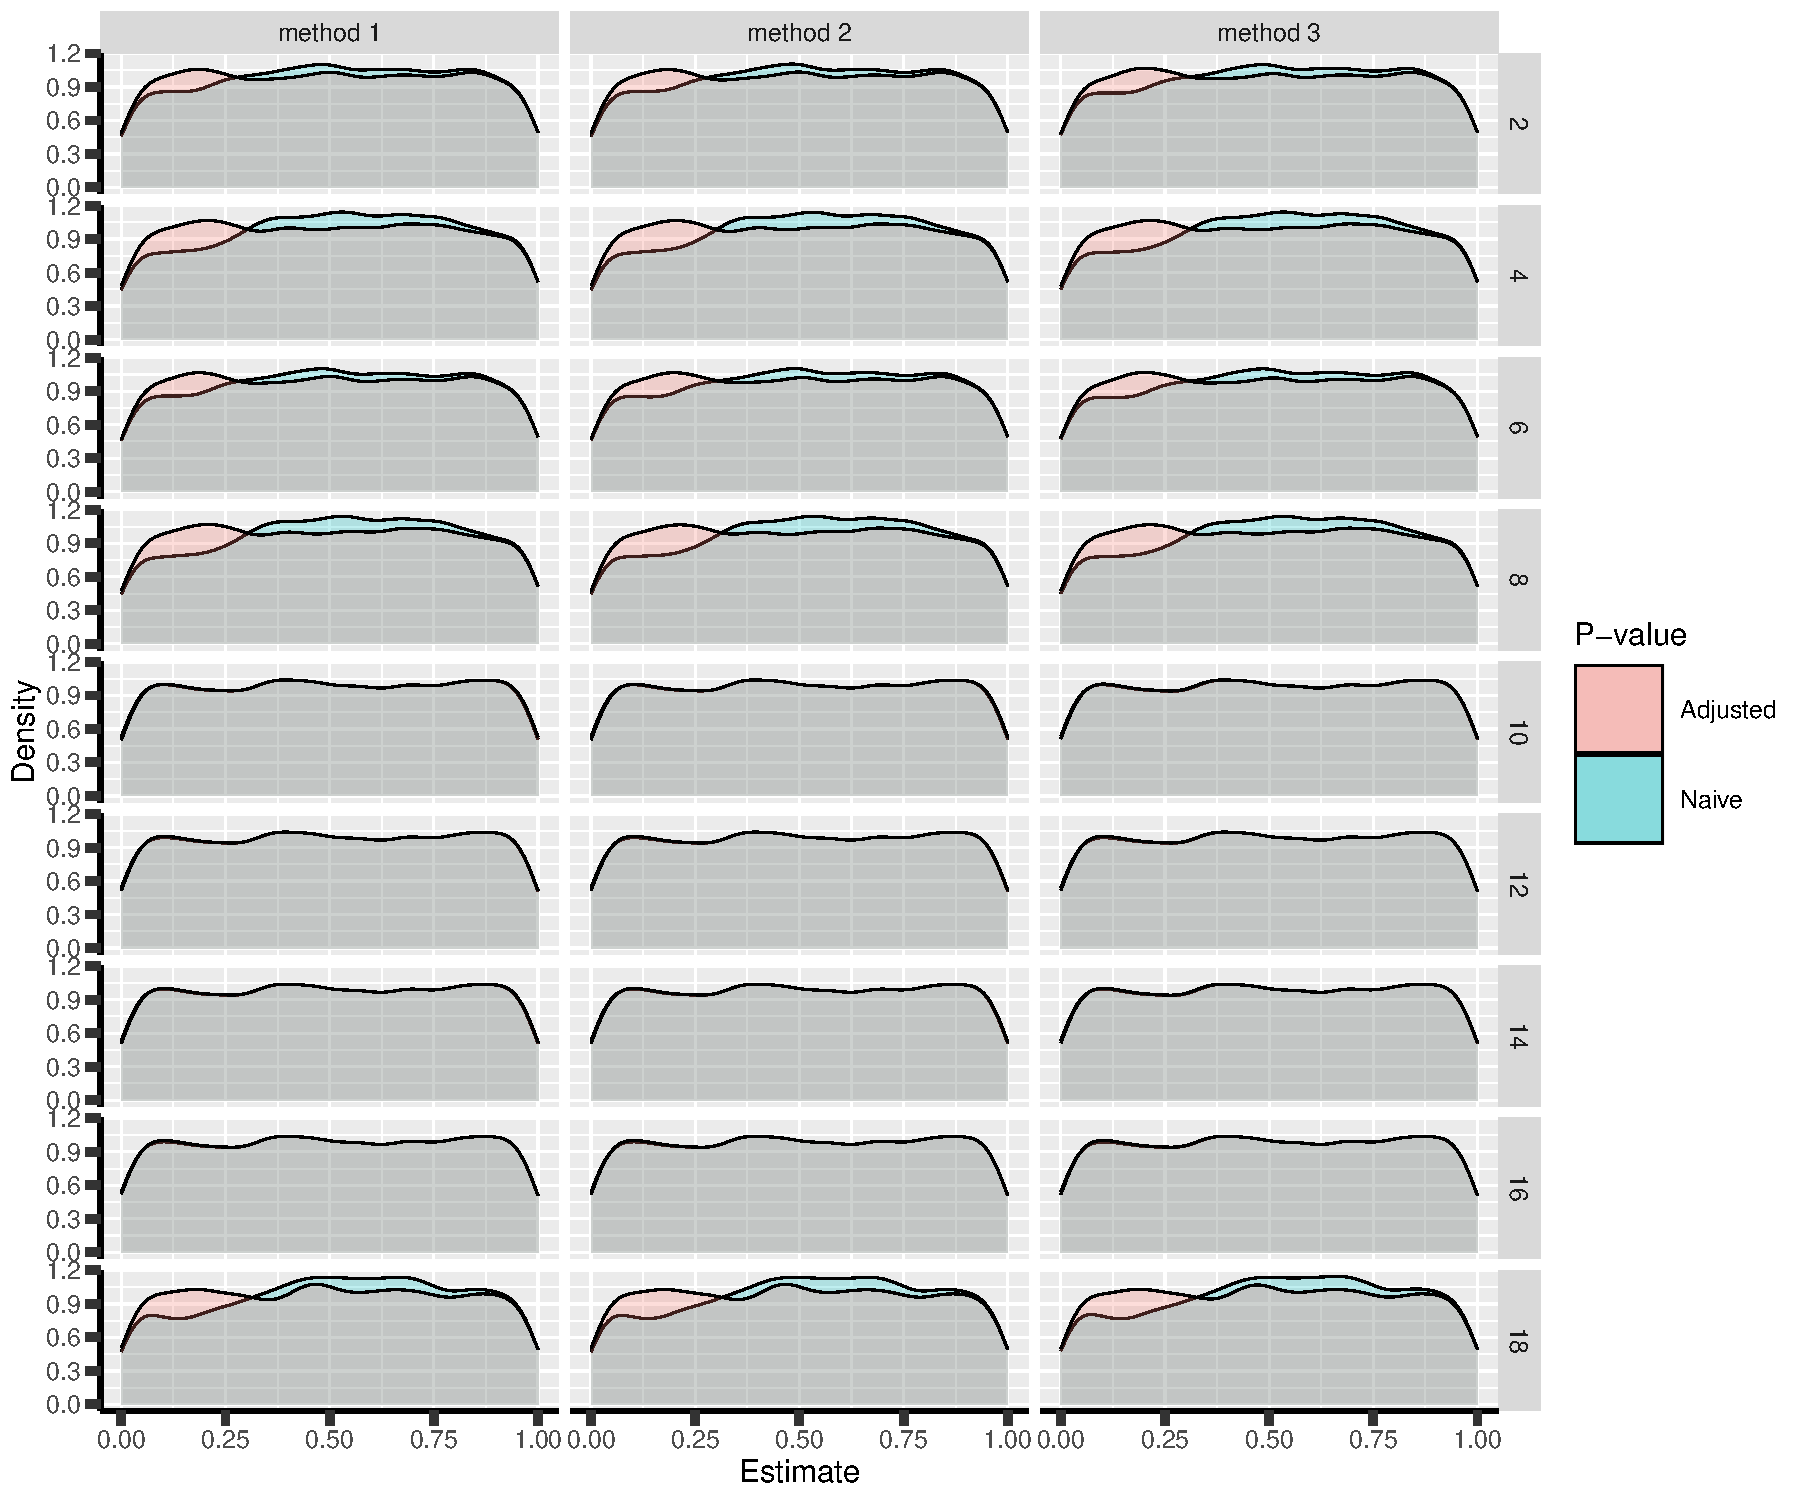
\includegraphics[trim={0 0 0 0},width=1\textwidth]{./figures/gg-pvalue-density.pdf}
\caption{Naive and adjusted p-value distribution over all simulations under the null. Each row correspond to a different scenario}
\end{figure}

\begin{figure}[!h]
\centering
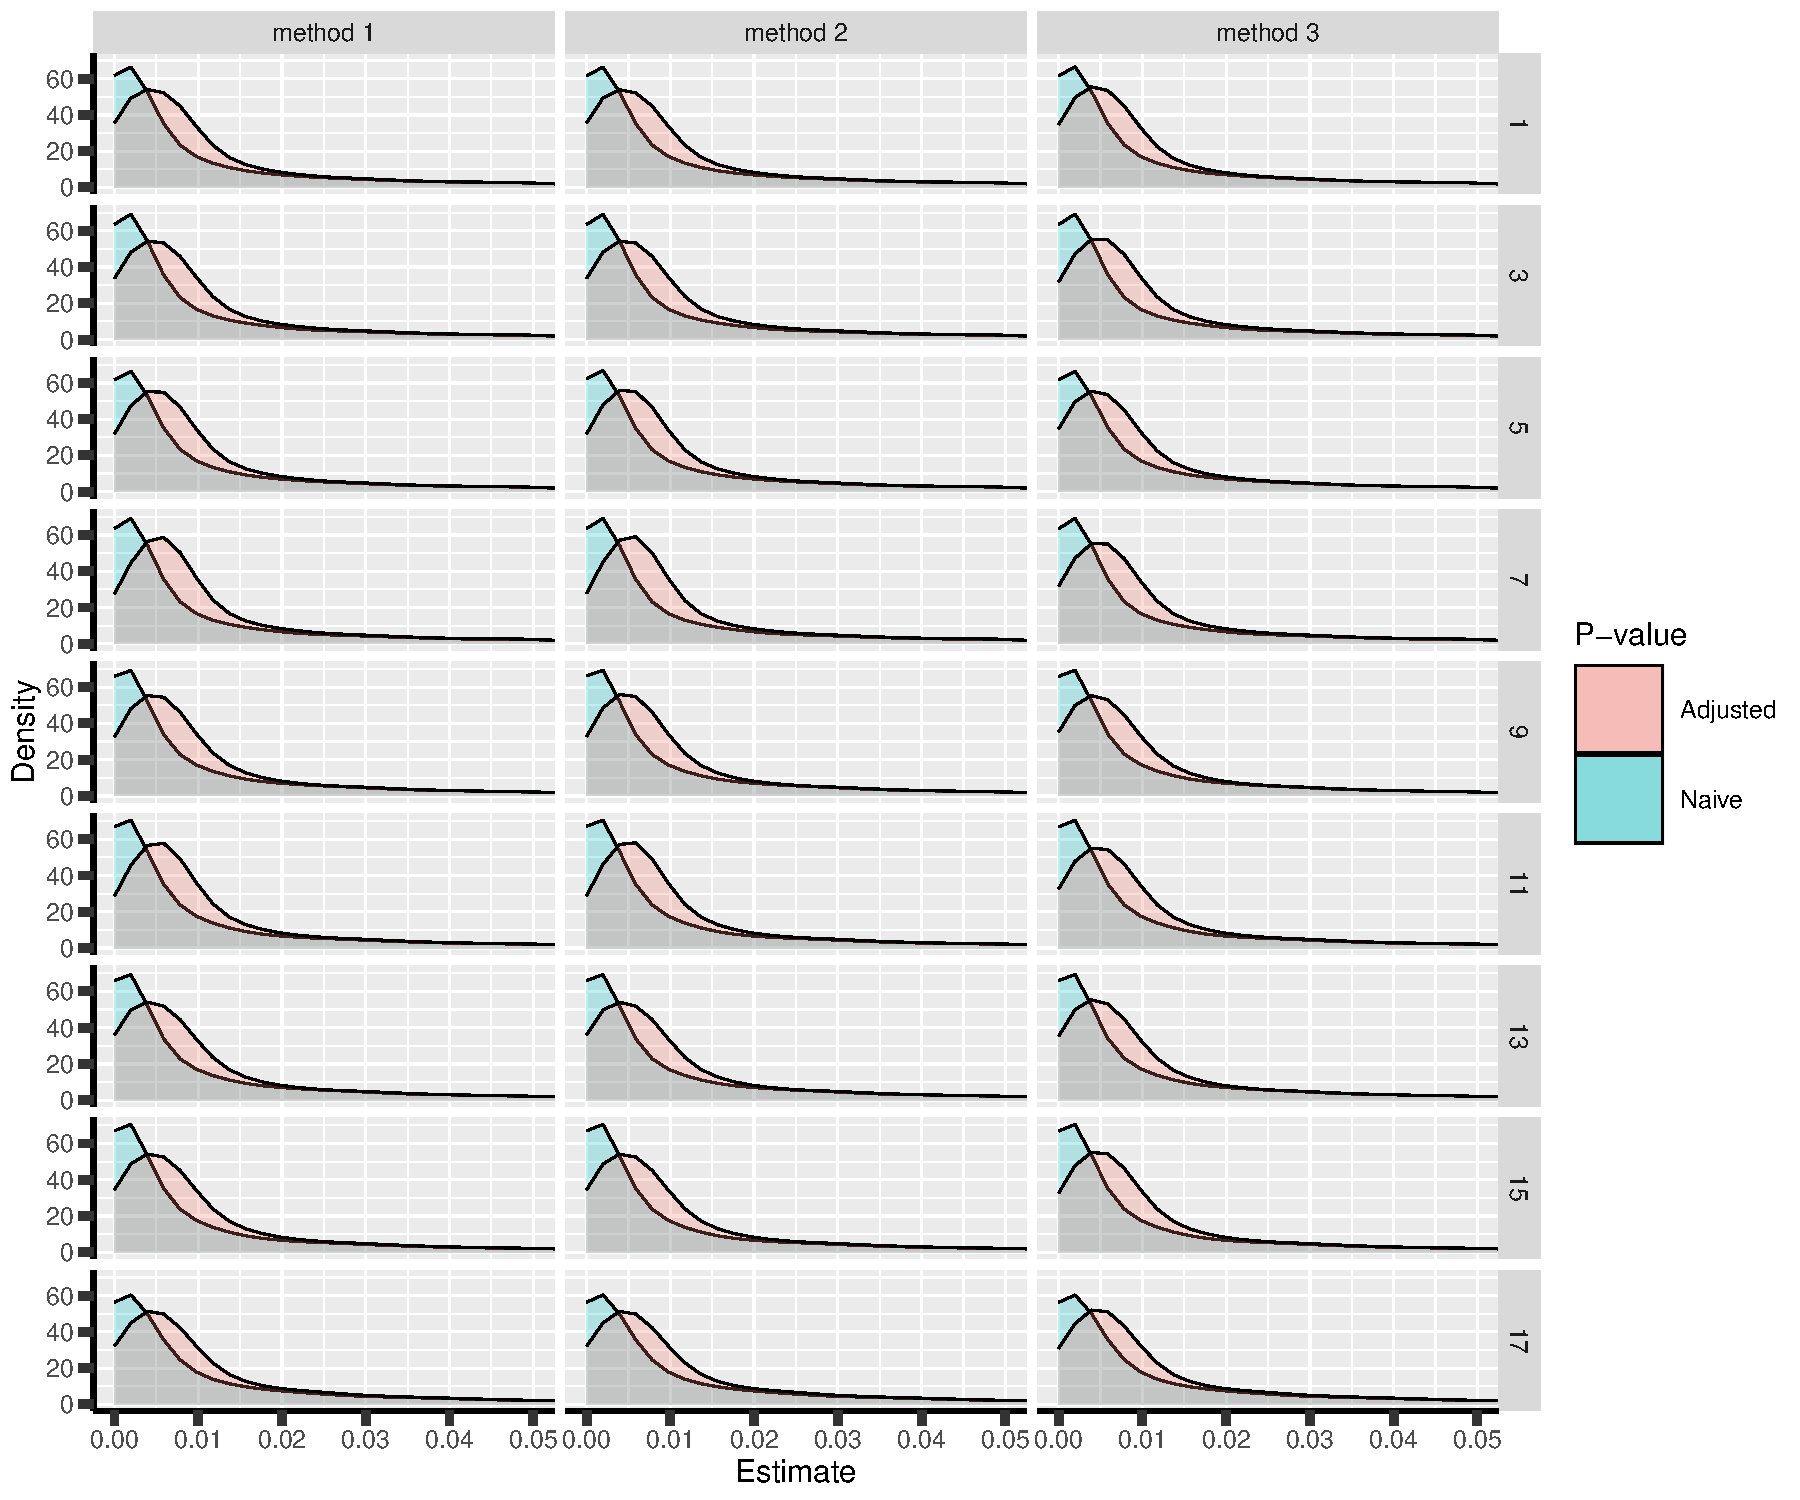
\includegraphics[trim={0 0 0 0},width=1\textwidth]{./figures/gg-pvalue2-density.pdf}
\caption{Naive and adjusted p-value distribution over all simulations under the alternative. Each row correspond to a different scenario}
\end{figure}

\clearpage

\section{Conclusion of the trial}
\label{sec:org4e56db1}

Relative frequency of stopping for efficacy/futility at decision/final

\begin{itemize}
\item Method 1
\end{itemize}
\begin{verbatim}
        N missing  hypo binding  fixC ar decision.eff decision.fut final.eff final.fut
 1: 10000    TRUE power    TRUE FALSE 10        37.79         5.93     43.21      13.1
 2: 10000    TRUE typeI    TRUE FALSE 10         0.80        71.13      1.62      26.5
 3: 10000    TRUE power    TRUE FALSE  5        35.74         5.98     44.79      13.5
 4: 10000    TRUE typeI    TRUE FALSE  5         0.74        69.32      1.66      28.3
 5: 10000    TRUE power    TRUE  TRUE 10        36.94         6.78     43.21      13.1
 6: 10000    TRUE typeI    TRUE  TRUE 10         0.62        71.31      1.62      26.5
 7: 10000    TRUE power    TRUE  TRUE  5        35.29         6.43     44.79      13.5
 8: 10000    TRUE typeI    TRUE  TRUE  5         0.66        69.40      1.66      28.3
 9: 10000    TRUE power   FALSE  TRUE 10        38.05         6.57     41.81      13.6
10: 10000    TRUE typeI   FALSE  TRUE 10         0.61         0.20      1.84      97.4
11: 10000    TRUE power   FALSE  TRUE  5        36.35         6.15     43.58      13.9
12: 10000    TRUE typeI   FALSE  TRUE  5         0.70         0.06      1.93      97.3
13: 10000    TRUE power   FALSE FALSE 10        38.69         5.93     41.81      13.6
14: 10000    TRUE typeI   FALSE FALSE 10         0.69         0.12      1.84      97.4
15: 10000    TRUE power   FALSE FALSE  5        36.79         5.71     43.58      13.9
16: 10000    TRUE typeI   FALSE FALSE  5         0.75         0.01      1.93      97.3
17: 10000   FALSE power    TRUE FALSE  5        33.98         5.33     46.33      14.4
18: 10000   FALSE typeI    TRUE FALSE  5         0.74        67.48      1.72      30.1
\end{verbatim}

\clearpage

Method 2:
\begin{verbatim}
        N missing  hypo binding  fixC ar decision.eff decision.fut final.eff final.fut
 1: 10000    TRUE power    TRUE FALSE 10        37.85         6.19     43.08      12.9
 2: 10000    TRUE typeI    TRUE FALSE 10         0.79        71.64      1.60      26.0
 3: 10000    TRUE power    TRUE FALSE  5        35.77         5.99     44.76      13.5
 4: 10000    TRUE typeI    TRUE FALSE  5         0.74        69.38      1.66      28.2
 5: 10000    TRUE power    TRUE  TRUE 10        36.69         6.24     43.66      13.4
 6: 10000    TRUE typeI    TRUE  TRUE 10         0.59        69.61      1.63      28.2
 7: 10000    TRUE power    TRUE  TRUE  5        35.02         6.05     45.18      13.8
 8: 10000    TRUE typeI    TRUE  TRUE  5         0.63        68.36      1.68      29.3
 9: 10000    TRUE power   FALSE  TRUE 10        37.85         6.04     42.27      13.8
10: 10000    TRUE typeI   FALSE  TRUE 10         0.61         0.19      1.86      97.3
11: 10000    TRUE power   FALSE  TRUE  5        36.18         5.84     43.86      14.1
12: 10000    TRUE typeI   FALSE  TRUE  5         0.69         0.06      1.95      97.3
13: 10000    TRUE power   FALSE FALSE 10        38.70         6.09     41.74      13.5
14: 10000    TRUE typeI   FALSE FALSE 10         0.69         0.12      1.84      97.4
15: 10000    TRUE power   FALSE FALSE  5        36.82         5.75     43.54      13.9
16: 10000    TRUE typeI   FALSE FALSE  5         0.75         0.01      1.93      97.3
17: 10000   FALSE power    TRUE FALSE  5        34.03         5.36     46.27      14.3
18: 10000   FALSE typeI    TRUE FALSE  5         0.74        67.55      1.72      30.0
\end{verbatim}

\clearpage

Method 3:
\begin{verbatim}
        N missing  hypo binding  fixC ar decision.eff decision.fut final.eff final.fut
 1: 10000    TRUE power    TRUE FALSE 10        40.58         6.53     39.85      13.0
 2: 10000    TRUE typeI    TRUE FALSE 10         0.74        68.79      1.63      28.8
 3: 10000    TRUE power    TRUE FALSE  5        36.54         6.30     43.60      13.6
 4: 10000    TRUE typeI    TRUE FALSE  5         0.69        68.41      1.66      29.2
 5: 10000    TRUE power    TRUE  TRUE 10        40.58         6.53     39.85      13.0
 6: 10000    TRUE typeI    TRUE  TRUE 10         0.74        68.79      1.63      28.8
 7: 10000    TRUE power    TRUE  TRUE  5        36.54         6.30     43.60      13.6
 8: 10000    TRUE typeI    TRUE  TRUE  5         0.69        68.41      1.66      29.2
 9: 10000    TRUE power   FALSE  TRUE 10        41.34         6.20     38.92      13.5
10: 10000    TRUE typeI   FALSE  TRUE 10         0.77         0.33      1.80      97.1
11: 10000    TRUE power   FALSE  TRUE  5        37.71         6.03     42.35      13.9
12: 10000    TRUE typeI   FALSE  TRUE  5         0.73         0.09      1.93      97.2
13: 10000    TRUE power   FALSE FALSE 10        41.34         6.20     38.92      13.5
14: 10000    TRUE typeI   FALSE FALSE 10         0.77         0.33      1.80      97.1
15: 10000    TRUE power   FALSE FALSE  5        37.71         6.03     42.35      13.9
16: 10000    TRUE typeI   FALSE FALSE  5         0.73         0.09      1.93      97.2
17: 10000   FALSE power    TRUE FALSE  5        34.65         5.59     45.27      14.5
18: 10000   FALSE typeI    TRUE FALSE  5         0.68        66.54      1.77      31.0
\end{verbatim}

\clearpage

\section{Bias (True effect: 0.6 under the alternative)}
\label{sec:org01885da}

Bias per estimator and method\footnote{e.g. \texttt{biasMLE1} mixed model
estimator (treatment effect), method 1 (boundaries)}:
\begin{adjustwidth}{-1cm}{-1cm}
\begin{verbatim}
     hypo missing binding  fixC ar  biasMLE1  biasMLE2  biasMLE3  biasMUE1  biasMUE2 biasMUE3
 1: power    TRUE    TRUE FALSE 10  0.013450  0.013150  0.014680  0.005983  0.005659  0.00218
 2: typeI    TRUE    TRUE FALSE 10 -0.017939 -0.017844 -0.018560 -0.004484 -0.004412 -0.00508
 3: power    TRUE    TRUE FALSE  5  0.022570  0.022551  0.023584  0.010450  0.010477  0.00870
 4: typeI    TRUE    TRUE FALSE  5 -0.030342 -0.030312 -0.030651 -0.011844 -0.011798 -0.01238
 5: power    TRUE    TRUE  TRUE 10  0.013450  0.014032  0.014680  0.001094  0.001687  0.00217
 6: typeI    TRUE    TRUE  TRUE 10 -0.017939 -0.018711 -0.018560 -0.005373 -0.006062 -0.00508
 7: power    TRUE    TRUE  TRUE  5  0.022570  0.023089  0.023584  0.007878  0.008275  0.00870
 8: typeI    TRUE    TRUE  TRUE  5 -0.030342 -0.030850 -0.030651 -0.012252 -0.012829 -0.01238
 9: power    TRUE   FALSE  TRUE 10  0.014326  0.014903  0.015285  0.037532  0.035615  0.03135
10: typeI    TRUE   FALSE  TRUE 10  0.000186  0.000192  0.000511  0.000991  0.000981  0.00263
11: power    TRUE   FALSE  TRUE  5  0.023657  0.024021  0.024379  0.042787  0.041614  0.04039
12: typeI    TRUE   FALSE  TRUE  5  0.000912  0.000853  0.001008  0.001112  0.001062  0.00136
13: power    TRUE   FALSE FALSE 10  0.014326  0.014160  0.015285  0.036631  0.037167  0.03139
14: typeI    TRUE   FALSE FALSE 10  0.000186  0.000186  0.000511  0.000793  0.000783  0.00264
15: power    TRUE   FALSE FALSE  5  0.023657  0.023651  0.024379  0.041744  0.041949  0.04040
16: typeI    TRUE   FALSE FALSE  5  0.000912  0.000912  0.001008  0.000964  0.000962  0.00137
17: power   FALSE    TRUE FALSE  5  0.022836  0.022775  0.023807  0.011971  0.011956  0.01001
18: typeI   FALSE    TRUE FALSE  5 -0.029516 -0.029448 -0.029915 -0.011048 -0.011005 -0.01162
\end{verbatim}
\end{adjustwidth}

Median bias \footnote{Relative frequency at which the estimate is greater than the truth minus 0.5} per estimator and method:
\begin{adjustwidth}{-1cm}{-1cm}
\begin{verbatim}
     hypo missing binding  fixC ar mbiasMLE1 mbiasMLE2 mbiasMLE3 mbiasMUE1 mbiasMUE2 mbiasMUE3
 1: power    TRUE    TRUE FALSE 10    0.0261    0.0260    0.0301   -0.0024   -0.0025   -0.0054
 2: typeI    TRUE    TRUE FALSE 10   -0.0173   -0.0170   -0.0202    0.0011    0.0009   -0.0001
 3: power    TRUE    TRUE FALSE  5    0.0405    0.0405    0.0432   -0.0034   -0.0033   -0.0053
 4: typeI    TRUE    TRUE FALSE  5   -0.0330   -0.0329   -0.0345    0.0007    0.0007    0.0008
 5: power    TRUE    TRUE  TRUE 10    0.0261    0.0265    0.0301   -0.0105   -0.0101   -0.0054
 6: typeI    TRUE    TRUE  TRUE 10   -0.0173   -0.0197   -0.0202    0.0011   -0.0006   -0.0001
 7: power    TRUE    TRUE  TRUE  5    0.0405    0.0407    0.0432   -0.0077   -0.0065   -0.0053
 8: typeI    TRUE    TRUE  TRUE  5   -0.0330   -0.0346   -0.0345    0.0007    0.0009    0.0008
 9: power    TRUE   FALSE  TRUE 10    0.0326    0.0332    0.0327    0.0390    0.0345    0.0277
10: typeI    TRUE   FALSE  TRUE 10   -0.0009   -0.0009   -0.0009   -0.0008   -0.0008    0.0014
11: power    TRUE   FALSE  TRUE  5    0.0462    0.0459    0.0489    0.0338    0.0315    0.0294
12: typeI    TRUE   FALSE  TRUE  5   -0.0009   -0.0010   -0.0009   -0.0008   -0.0010    0.0003
13: power    TRUE   FALSE FALSE 10    0.0326    0.0324    0.0327    0.0390    0.0403    0.0277
14: typeI    TRUE   FALSE FALSE 10   -0.0009   -0.0009   -0.0009   -0.0008   -0.0008    0.0014
15: power    TRUE   FALSE FALSE  5    0.0462    0.0464    0.0489    0.0337    0.0342    0.0294
16: typeI    TRUE   FALSE FALSE  5   -0.0009   -0.0009   -0.0009   -0.0008   -0.0008    0.0003
17: power   FALSE    TRUE FALSE  5    0.0383    0.0383    0.0400   -0.0026   -0.0025   -0.0047
18: typeI   FALSE    TRUE FALSE  5   -0.0329   -0.0327   -0.0353    0.0044    0.0044    0.0035
\end{verbatim}

\end{adjustwidth}

\clearpage

\section{Distribution of the estimates}
\label{sec:orgea1e4f0}

Distribution of the estimates:
\begin{figure}[!h]
\centering
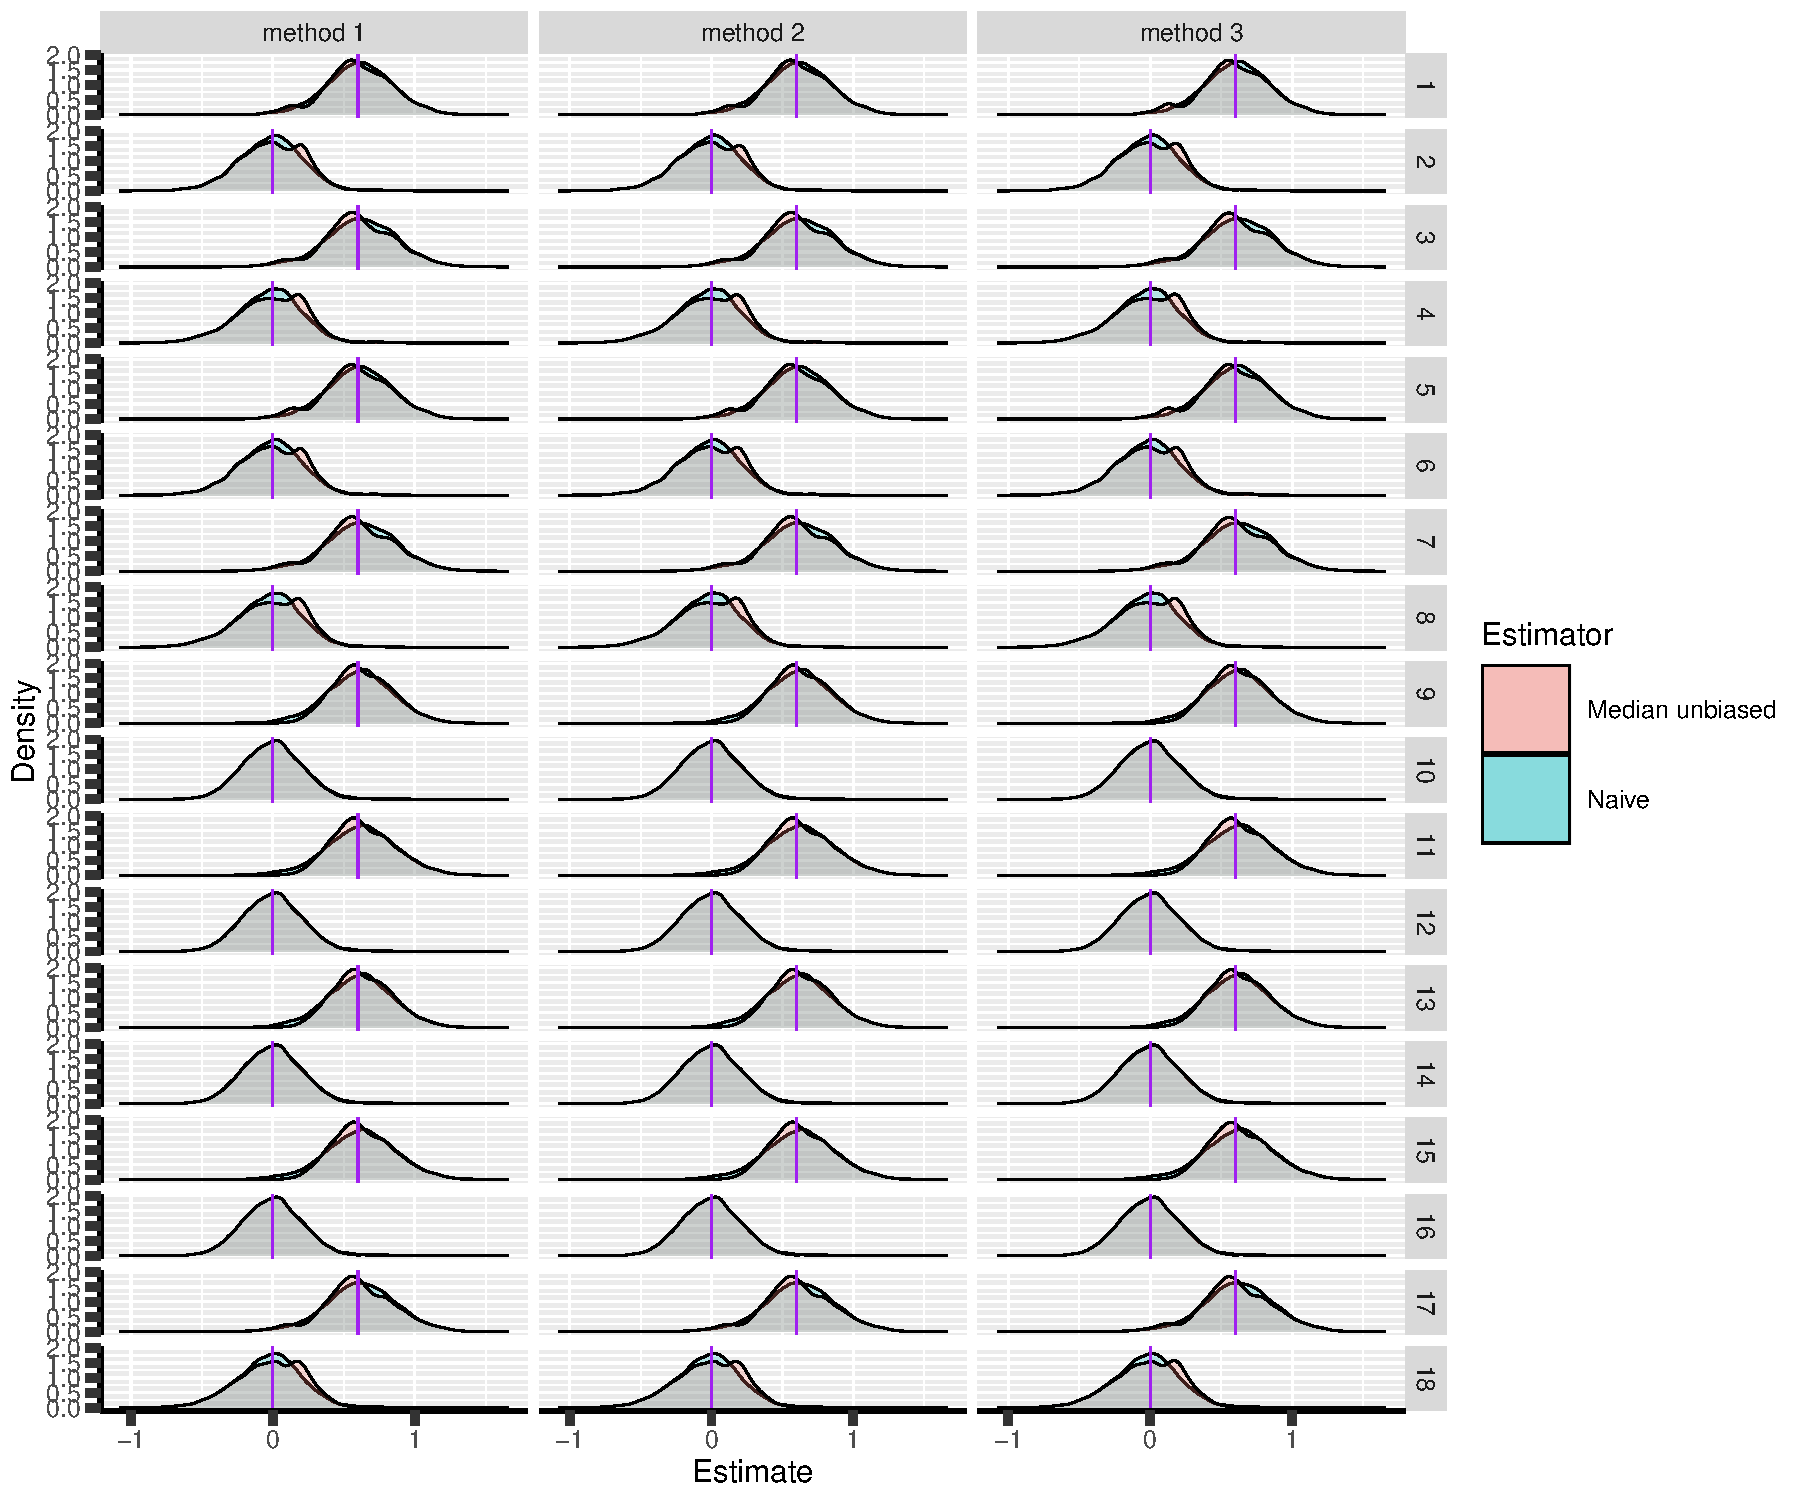
\includegraphics[trim={0 0 0 0},width=1\textwidth]{./figures/gg-estimate-density.pdf}
\caption{Naive and Median unbiased estimate distribution over all simulations. Each row correspond to a different scenario}
\end{figure}

\begin{figure}[!h]
\centering
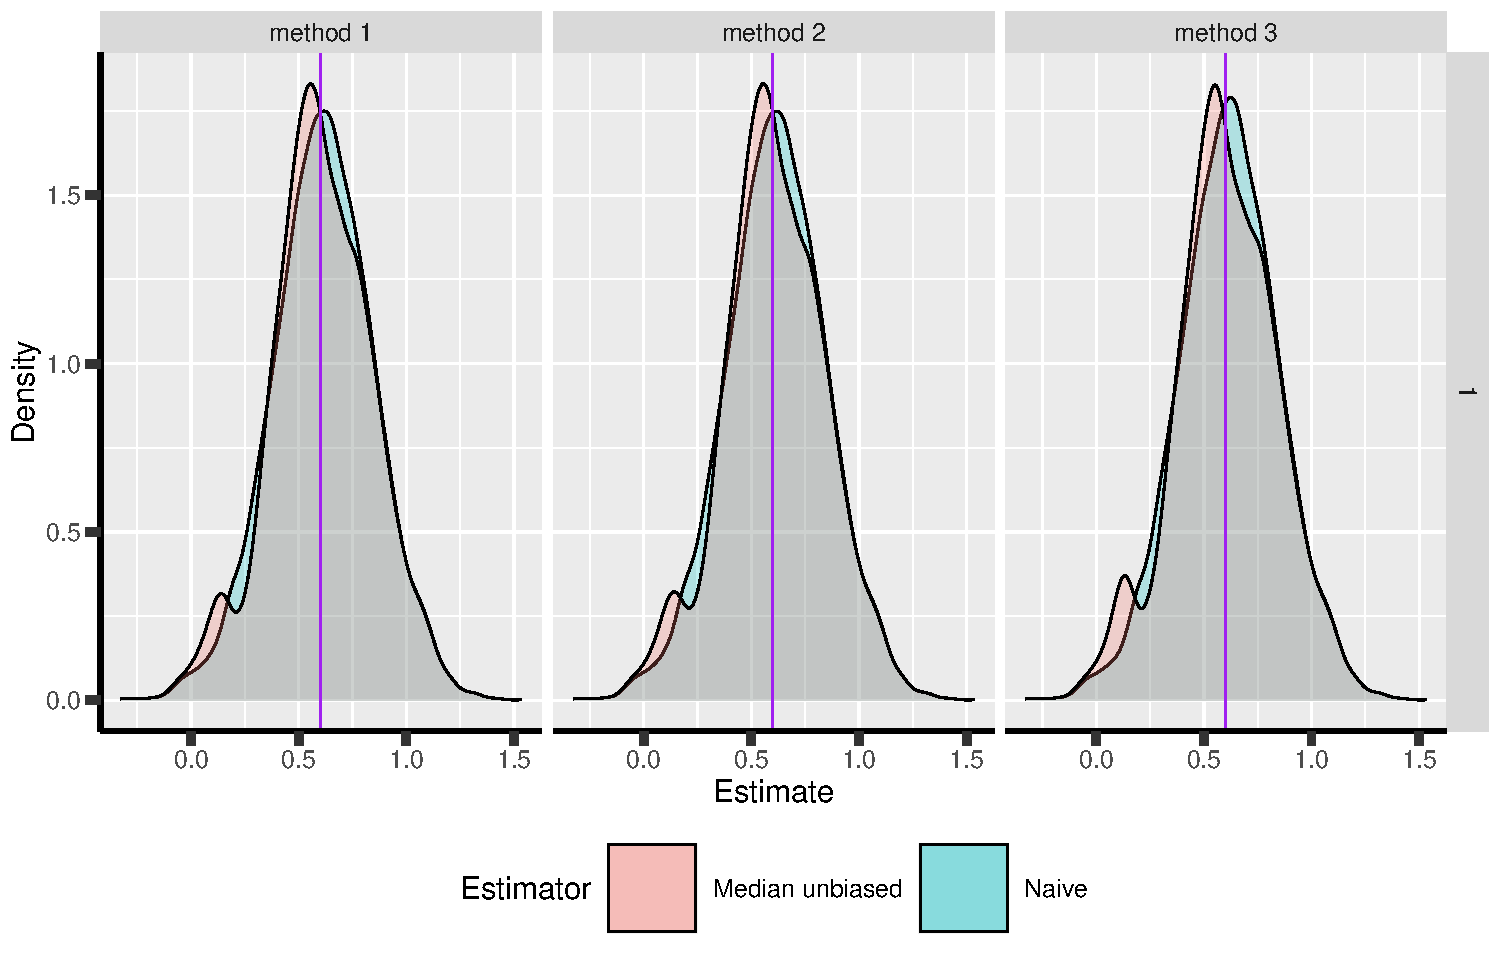
\includegraphics[trim={0 0 0 0},width=\textwidth]{./figures/gg-estimate-density-scenario1.pdf}
\caption{Same but specific to scenario 1}
\end{figure}

\clearpage

Distribution of the median unbiased estimate conditional to the stage:
\begin{figure}[!h]
\centering
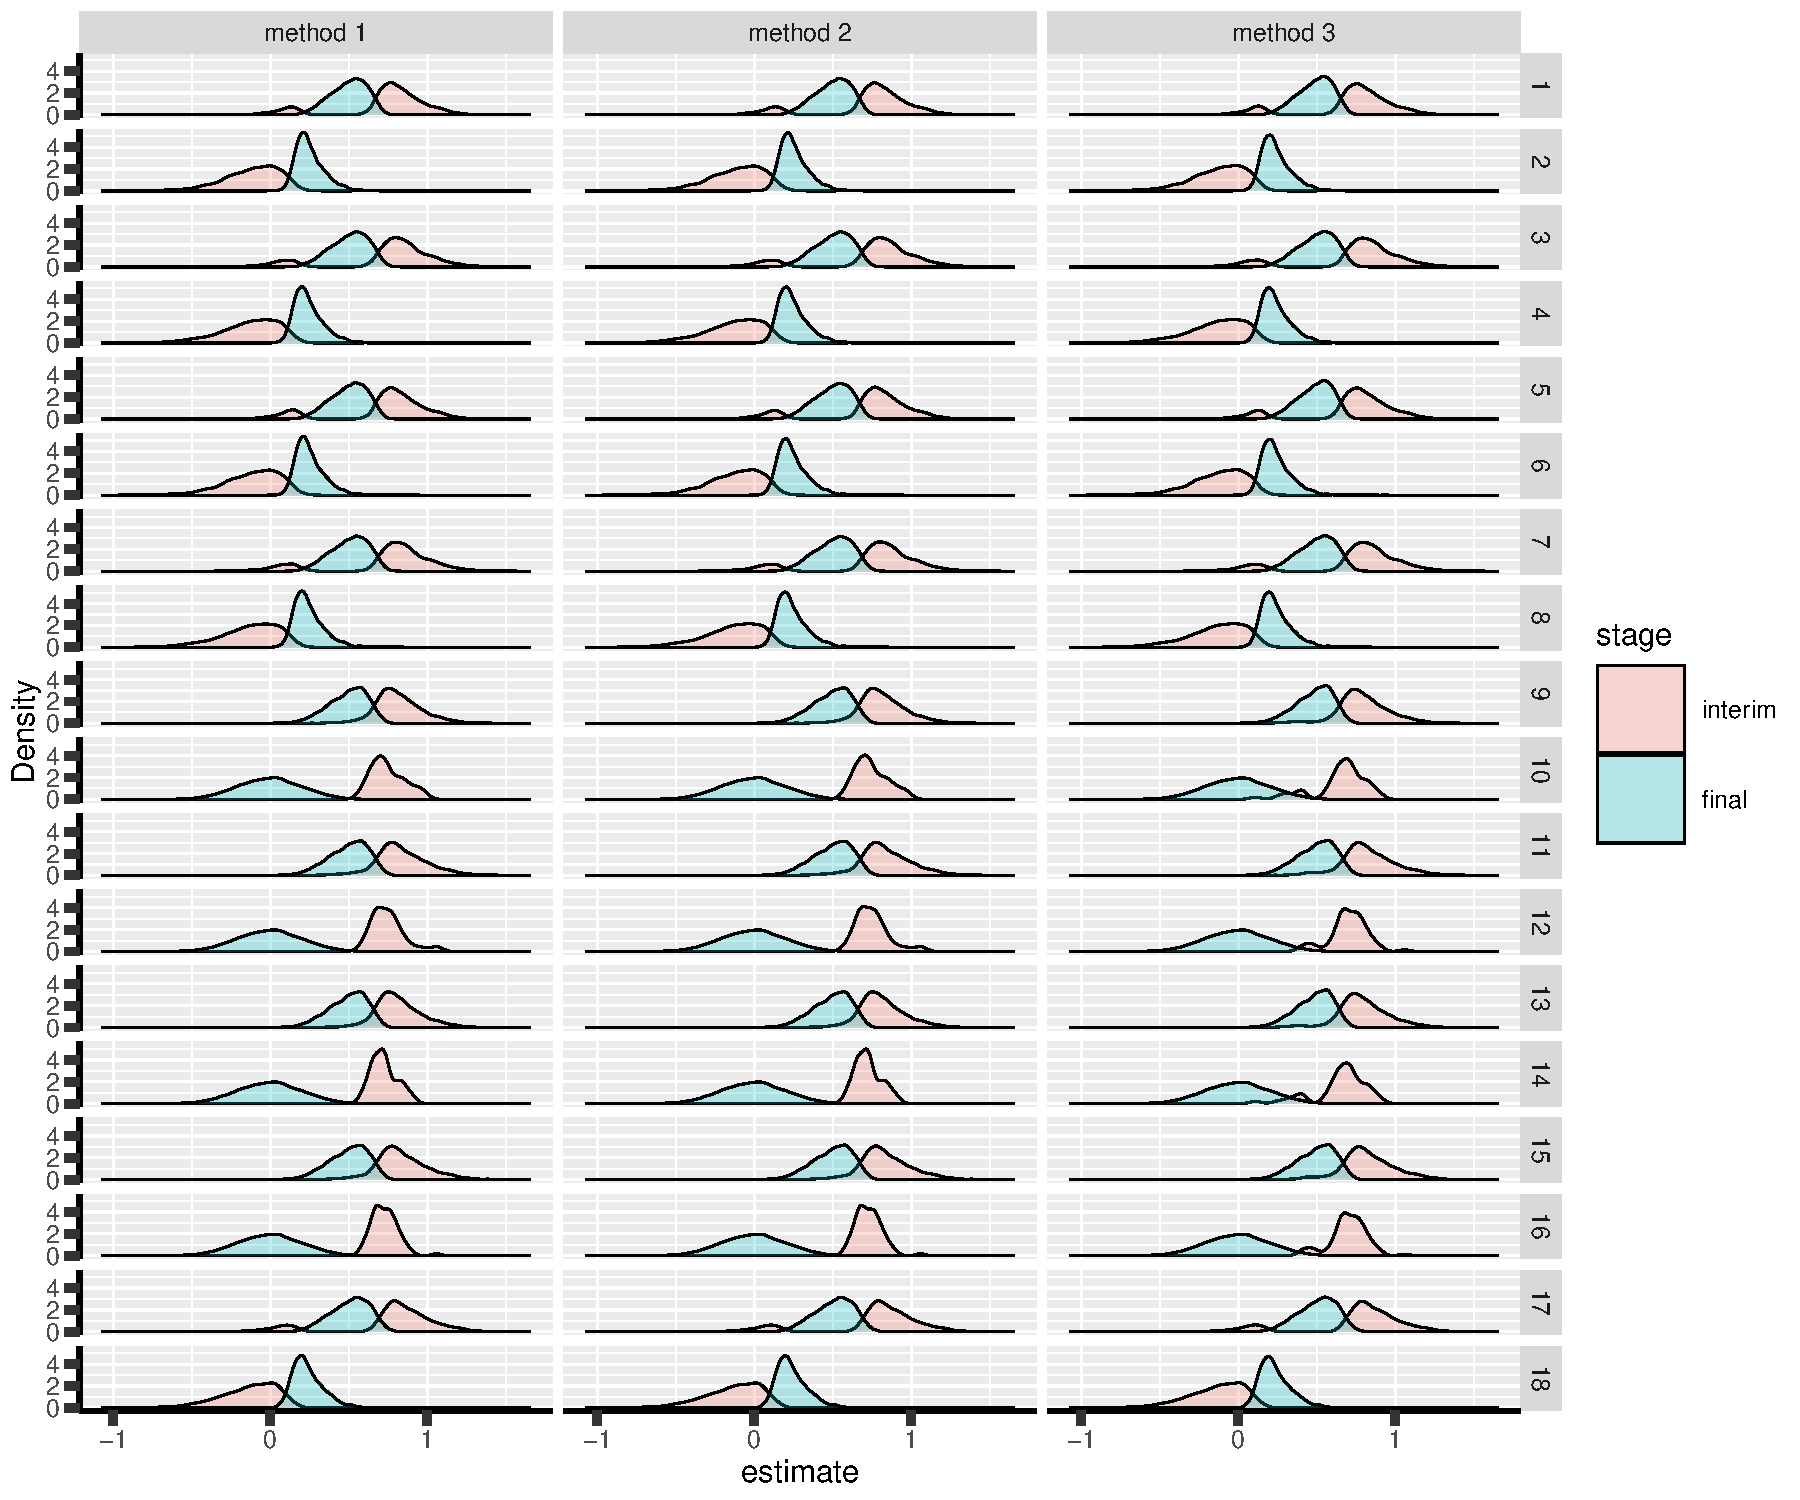
\includegraphics[trim={0 0 0 0},width=1\textwidth]{./figures/gg-estimateC-density.pdf}
\caption{Median unbiased estimate distribution conditional to the stage. Each row correspond to a different scenario.}
\end{figure}

\clearpage

\section{Special cases}
\label{sec:orgcefa52e}

Reason for stopping (efficacy, futility, Imax reached), continuing the
trial (decreasing information, no boundary crossed), or concluding
(stop for futility at interim):
\begin{verbatim}
                                    scenario    1    2    3    4    5    6    7    8
reason                       method                                                 
decreasing information       1                  0    0    1    1    0    0    1    1
                             2                  0    0    1    1    0    0    1    1
                             3                  0    0    1    1    0    0    1    1
efficacy                     1               3739   81 3573   74 3739   81 3573   74
                             2               3744   81 3576   74 3718   79 3545   71
                             3               4165  108 3721   82 4165  108 3721   82
futility                     1                632 7111  599 6932  632 7111  599 6932
                             2                659 7161  600 6938  574 6940  562 6828
                             3                545 6844  563 6828  545 6844  563 6828
Imax reached                 1                  1    1    0    0    1    1    0    0
                             2                  1    1    0    0    1    1    0    0
                             3                  1    1    0    0    1    1    0    0
no boundary crossed          1               5628 2807 5828 2994 5628 2807 5828 2994
                             2               5596 2757 5824 2988 5707 2980 5893 3101
                             3               5289 3047 5716 3090 5289 3047 5716 3090
stop for futility at interim 1                  0    0    0    0    0    0    0    0
                             2                  0    0    0    0    0    0    0    0
                             3                 11    1    2    0   11    1    2    0
\end{verbatim}

\begin{verbatim}
                                    scenario    9   10   11   12   13   14   15   16   17   18
reason                       method                                                           
efficacy                     1               3849   81 3680   76 3849   81 3680   76 3396   74
                             2               3829   80 3661   75 3850   81 3683   76 3400   74
                             3               4238  110 3831   82 4238  110 3831   82 3528   80
futility                     1                613 7122  570 6945  613 7122  570 6945  535 6748
                             2                560 6975  541 6838  629 7164  574 6950  539 6755
                             3                516 6890  543 6842  516 6890  543 6842  496 6642
no boundary crossed          1               5538 2797 5750 2979 5538 2797 5750 2979 6069 3178
                             2               5611 2945 5798 3087 5521 2755 5743 2974 6061 3171
                             3               5246 3000 5626 3076 5246 3000 5626 3076 5976 3278
stop for futility at interim 1                  0    0    0    0    0    0    0    0    0    0
                             2                  0    0    0    0    0    0    0    0    0    0
                             3                  8    0    0    0    8    0    0    0    1    0
\end{verbatim}

\clearpage

\section{Reversal probability}
\label{sec:orge17b4b8}

Percentage of time we observe a reversal:
\begin{adjustwidth}{-1cm}{-1cm}
\begin{verbatim}
        N  hypo missing ar binding  fixC fu2eff_1 fu2eff_2 fu2eff_3 eff2fu_1 eff2fu_2 eff2fu_3
 1: 10000 power    TRUE 10    TRUE FALSE     0.57     0.61        0     0.17     0.20     1.07
 2: 10000 typeI    TRUE 10    TRUE FALSE     0.10     0.09        0     0.11     0.11     0.34
 3: 10000 power    TRUE  5    TRUE FALSE     0.08     0.08        0     0.07     0.07     0.67
 4: 10000 typeI    TRUE  5    TRUE FALSE     0.02     0.02        0     0.02     0.02     0.13
 5: 10000 power    TRUE 10    TRUE  TRUE     0.22     0.16        0     0.67     0.65     1.07
 6: 10000 typeI    TRUE 10    TRUE  TRUE     0.02     0.01        0     0.21     0.21     0.34
 7: 10000 power    TRUE  5    TRUE  TRUE     0.02     0.02        0     0.46     0.45     0.67
 8: 10000 typeI    TRUE  5    TRUE  TRUE     0.00     0.00        0     0.08     0.08     0.13
 9: 10000 power    TRUE 10   FALSE  TRUE     0.14     0.11        0     0.58     0.55     1.04
10: 10000 typeI    TRUE 10   FALSE  TRUE     0.00     0.00        0     0.20     0.19     0.33
11: 10000 power    TRUE  5   FALSE  TRUE     0.01     0.01        0     0.46     0.44     0.60
12: 10000 typeI    TRUE  5   FALSE  TRUE     0.00     0.00        0     0.06     0.06     0.09
13: 10000 power    TRUE 10   FALSE FALSE     0.41     0.42        0     0.21     0.22     1.04
14: 10000 typeI    TRUE 10   FALSE FALSE     0.00     0.00        0     0.12     0.12     0.33
15: 10000 power    TRUE  5   FALSE FALSE     0.03     0.03        0     0.04     0.04     0.60
16: 10000 typeI    TRUE  5   FALSE FALSE     0.00     0.00        0     0.01     0.01     0.09
17: 10000 power   FALSE  5    TRUE FALSE     0.06     0.07        0     0.04     0.04     0.63
18: 10000 typeI   FALSE  5    TRUE FALSE     0.01     0.01        0     0.01     0.01     0.12
\end{verbatim}

\end{adjustwidth}


\clearpage

\section{Logical consistency of p-values/CIs}
\label{sec:org5292659}

\subsection{Mismatch p-value / boundaries}
\label{sec:orgafa7ea3}

When concluding for futility:
\begin{verbatim}
     hypo missing ar binding  fixC method 1 method 2 method 3
 1: power    TRUE 10    TRUE FALSE        0        0        0
 2: typeI    TRUE 10    TRUE FALSE        0        0        0
 3: power    TRUE  5    TRUE FALSE        0        0        0
 4: typeI    TRUE  5    TRUE FALSE        0        0        0
 5: power    TRUE 10    TRUE  TRUE        0        0        0
 6: typeI    TRUE 10    TRUE  TRUE        0        0        0
 7: power    TRUE  5    TRUE  TRUE        0        0        0
 8: typeI    TRUE  5    TRUE  TRUE        0        0        0
 9: power    TRUE 10   FALSE  TRUE        0        0        0
10: typeI    TRUE 10   FALSE  TRUE        0        0        0
11: power    TRUE  5   FALSE  TRUE        0        0        0
12: typeI    TRUE  5   FALSE  TRUE        0        0        0
13: power    TRUE 10   FALSE FALSE        0        0        0
14: typeI    TRUE 10   FALSE FALSE        0        0        0
15: power    TRUE  5   FALSE FALSE        0        0        0
16: typeI    TRUE  5   FALSE FALSE        0        0        0
17: power   FALSE  5    TRUE FALSE        0        0        0
18: typeI   FALSE  5    TRUE FALSE        0        0        0
\end{verbatim}

When concluding for efficacy:
\begin{verbatim}
     hypo missing ar binding  fixC method 1 method 2 method 3
 1: power    TRUE 10    TRUE FALSE        0        0        0
 2: typeI    TRUE 10    TRUE FALSE        0        0        0
 3: power    TRUE  5    TRUE FALSE        0        0        0
 4: typeI    TRUE  5    TRUE FALSE        0        0        0
 5: power    TRUE 10    TRUE  TRUE        0        0        0
 6: typeI    TRUE 10    TRUE  TRUE        0        0        0
 7: power    TRUE  5    TRUE  TRUE        0        0        0
 8: typeI    TRUE  5    TRUE  TRUE        0        0        0
 9: power    TRUE 10   FALSE  TRUE        0        0        0
10: typeI    TRUE 10   FALSE  TRUE        0        0        0
11: power    TRUE  5   FALSE  TRUE        0        0        0
12: typeI    TRUE  5   FALSE  TRUE        0        0        0
13: power    TRUE 10   FALSE FALSE        0        0        0
14: typeI    TRUE 10   FALSE FALSE        0        0        0
15: power    TRUE  5   FALSE FALSE        0        0        0
16: typeI    TRUE  5   FALSE FALSE        0        0        0
17: power   FALSE  5    TRUE FALSE        0        0        0
18: typeI   FALSE  5    TRUE FALSE        0        0        0
\end{verbatim}

\clearpage

\subsection{Mismatch confidence intervals / boundaries}
\label{sec:org5b21698}

When concluding for futility:
\begin{verbatim}
     hypo missing ar binding  fixC method 1 method 2  method 3
 1: power    TRUE 10    TRUE FALSE        0        0 0.0000000
 2: typeI    TRUE 10    TRUE FALSE        0        0 0.0000000
 3: power    TRUE  5    TRUE FALSE        0        0 0.0000000
 4: typeI    TRUE  5    TRUE FALSE        0        0 0.0000000
 5: power    TRUE 10    TRUE  TRUE        0        0 0.0000000
 6: typeI    TRUE 10    TRUE  TRUE        0        0 0.0000000
 7: power    TRUE  5    TRUE  TRUE        0        0 0.0000000
 8: typeI    TRUE  5    TRUE  TRUE        0        0 0.0000000
 9: power    TRUE 10   FALSE  TRUE        0        0 7.8484438
10: typeI    TRUE 10   FALSE  TRUE        0        0 0.1747533
11: power    TRUE  5   FALSE  TRUE        0        0 4.1322314
12: typeI    TRUE  5   FALSE  TRUE        0        0 0.0821946
13: power    TRUE 10   FALSE FALSE        0        0 7.8484438
14: typeI    TRUE 10   FALSE FALSE        0        0 0.1747533
15: power    TRUE  5   FALSE FALSE        0        0 4.1322314
16: typeI    TRUE  5   FALSE FALSE        0        0 0.0821946
17: power   FALSE  5    TRUE FALSE        0        0 0.0000000
18: typeI   FALSE  5    TRUE FALSE        0        0 0.0000000
\end{verbatim}

This only occurs for non-binding futility rules and concluding futility, e.g.:
\#+END\textsubscript{SRC}


When concluding for efficacy:
\begin{verbatim}
     hypo missing ar binding  fixC method 1 method 2 method 3
 1: power    TRUE 10    TRUE FALSE        0        0        0
 2: typeI    TRUE 10    TRUE FALSE        0        0        0
 3: power    TRUE  5    TRUE FALSE        0        0        0
 4: typeI    TRUE  5    TRUE FALSE        0        0        0
 5: power    TRUE 10    TRUE  TRUE        0        0        0
 6: typeI    TRUE 10    TRUE  TRUE        0        0        0
 7: power    TRUE  5    TRUE  TRUE        0        0        0
 8: typeI    TRUE  5    TRUE  TRUE        0        0        0
 9: power    TRUE 10   FALSE  TRUE        0        0        0
10: typeI    TRUE 10   FALSE  TRUE        0        0        0
11: power    TRUE  5   FALSE  TRUE        0        0        0
12: typeI    TRUE  5   FALSE  TRUE        0        0        0
13: power    TRUE 10   FALSE FALSE        0        0        0
14: typeI    TRUE 10   FALSE FALSE        0        0        0
15: power    TRUE  5   FALSE FALSE        0        0        0
16: typeI    TRUE  5   FALSE FALSE        0        0        0
17: power   FALSE  5    TRUE FALSE        0        0        0
18: typeI   FALSE  5    TRUE FALSE        0        0        0
\end{verbatim}

\subsection{Range of p-values}
\label{sec:org8d81157}

\begin{verbatim}
    missing binding  fixC ar  hypo        method 1        method 2       method 3
 1:    TRUE    TRUE FALSE 10 power      [0;0.9147]      [0;0.9147]     [0;0.9147]
 2:    TRUE    TRUE FALSE 10 typeI  [1e-04;0.9999]  [1e-04;0.9999] [1e-04;0.9999]
 3:    TRUE    TRUE FALSE  5 power      [0;0.9015]      [0;0.9015]     [0;0.9015]
 4:    TRUE    TRUE FALSE  5 typeI  [1e-04;0.9998]  [1e-04;0.9998] [1e-04;0.9998]
 5:    TRUE    TRUE  TRUE 10 power  [7e-04;0.9147]  [7e-04;0.9147]     [0;0.9147]
 6:    TRUE    TRUE  TRUE 10 typeI [0.0016;0.9999] [0.0016;0.9999] [1e-04;0.9999]
 7:    TRUE    TRUE  TRUE  5 power  [1e-04;0.9015]  [1e-04;0.9015]     [0;0.9015]
 8:    TRUE    TRUE  TRUE  5 typeI  [5e-04;0.9998]  [5e-04;0.9998] [1e-04;0.9998]
 9:    TRUE   FALSE  TRUE 10 power       [8e-04;1]       [8e-04;1]          [0;1]
10:    TRUE   FALSE  TRUE 10 typeI      [0.0015;1]      [0.0015;1]      [5e-04;1]
11:    TRUE   FALSE  TRUE  5 power       [1e-04;1]       [1e-04;1]          [0;1]
12:    TRUE   FALSE  TRUE  5 typeI       [6e-04;1]       [5e-04;1]      [2e-04;1]
13:    TRUE   FALSE FALSE 10 power           [0;1]           [0;1]          [0;1]
14:    TRUE   FALSE FALSE 10 typeI       [1e-04;1]       [1e-04;1]      [5e-04;1]
15:    TRUE   FALSE FALSE  5 power           [0;1]           [0;1]          [0;1]
16:    TRUE   FALSE FALSE  5 typeI           [0;1]           [0;1]      [2e-04;1]
17:   FALSE    TRUE FALSE  5 power      [0;0.9642]      [0;0.9642]     [0;0.9642]
18:   FALSE    TRUE FALSE  5 typeI           [0;1]           [0;1]      [3e-04;1]
\end{verbatim}

\section{Coverage}
\label{sec:org7ec3dc9}

Average width of the confidence intervals
\lstset{language=r,label= ,caption= ,captionpos=b,numbers=none}
\begin{lstlisting}
res2stage.width <- res2stage[decision %in% c("futility","efficacy"),
                             .(N = .N,
                               width.naive = mean(upper_ML-lower_ML, na.rm = TRUE),
                               width.MUE = mean(upper_MUE-lower_MUE, na.rm = TRUE)),
                             by = c("method.char","missing","binding","fixC","ar","hypo")]
res2stage.width[, width.ratio := width.MUE/width.naive]
dcast(res2stage.width, hypo + missing + ar + binding + fixC ~ method.char, value.var = "width.ratio")
\end{lstlisting}

\begin{verbatim}
     hypo missing ar binding  fixC  method 1  method 2 method 3
 1: power   FALSE  5    TRUE FALSE 1.0517981 1.0518066 1.053592
 2: power    TRUE  5   FALSE FALSE 1.0355785 1.0355525 1.030753
 3: power    TRUE  5   FALSE  TRUE 1.0410966 1.0414270 1.030753
 4: power    TRUE  5    TRUE FALSE 1.0513207 1.0513607 1.052634
 5: power    TRUE  5    TRUE  TRUE 1.0570088 1.0563598 1.052629
 6: power    TRUE 10   FALSE FALSE 1.0469276 1.0468858 1.039428
 7: power    TRUE 10   FALSE  TRUE 1.0634581 1.0625586 1.039438
 8: power    TRUE 10    TRUE FALSE 1.0624494 1.0626858 1.062576
 9: power    TRUE 10    TRUE  TRUE 1.0765867 1.0753692 1.062555
10: typeI   FALSE  5    TRUE FALSE 1.0431774 1.0431218 1.046821
11: typeI    TRUE  5   FALSE FALSE 0.9997886 0.9998440 1.018905
12: typeI    TRUE  5   FALSE  TRUE 0.9996979 0.9996859 1.018905
13: typeI    TRUE  5    TRUE FALSE 1.0416221 1.0415882 1.045180
14: typeI    TRUE  5    TRUE  TRUE 1.0416986 1.0423673 1.045180
15: typeI    TRUE 10   FALSE FALSE 1.0182710 1.0227130 1.049875
16: typeI    TRUE 10   FALSE  TRUE 1.0183637 1.0101640 1.049882
17: typeI    TRUE 10    TRUE FALSE 1.0459447 1.0453954 1.056218
18: typeI    TRUE 10    TRUE  TRUE 1.0461003 1.0478314 1.056215
\end{verbatim}

\section{Percentage of missing values}
\label{sec:org911d30a}

Here only for method 1 - values are very similar between different
methods:
\begin{itemize}
\item \texttt{pc.all} percentage of observations with full data
\item \texttt{pc.missing3} percentage of observations missing the final outcome
but with intermediate outcome value and baseline.
\item \texttt{pc.missing23} percentage of observations with only baseline value
\end{itemize}
\begin{verbatim}
    method missing ar  hypo  fixC binding     N   pc.all pc.missing3 pc.missing23
 1:      1    TRUE  5 power FALSE    TRUE 10000 79.52088    9.591086    10.888036
 2:      1    TRUE  5 typeI FALSE    TRUE 10000 79.52088    9.591086    10.888036
 3:      1    TRUE  5 power  TRUE    TRUE 10000 79.52088    9.591086    10.888036
 4:      1    TRUE  5 typeI  TRUE    TRUE 10000 79.52088    9.591086    10.888036
 5:      1    TRUE  5 power  TRUE   FALSE 10000 79.64470    9.441772    10.913523
 6:      1    TRUE  5 typeI  TRUE   FALSE 10000 79.64470    9.441772    10.913523
 7:      1    TRUE  5 power FALSE   FALSE 10000 79.64470    9.441772    10.913523
 8:      1    TRUE  5 typeI FALSE   FALSE 10000 79.64470    9.441772    10.913523
 9:      1   FALSE  5 power FALSE    TRUE 10000 87.78863    6.090240     6.121126
10:      1   FALSE  5 typeI FALSE    TRUE 10000 87.78863    6.090240     6.121126
11:      1    TRUE 10 power FALSE    TRUE 10000 71.59741   13.353880    15.048710
12:      1    TRUE 10 typeI FALSE    TRUE 10000 71.59741   13.353880    15.048710
13:      1    TRUE 10 power  TRUE    TRUE 10000 71.59741   13.353880    15.048710
14:      1    TRUE 10 typeI  TRUE    TRUE 10000 71.59741   13.353880    15.048710
15:      1    TRUE 10 power  TRUE   FALSE 10000 71.79650   13.161615    15.041889
16:      1    TRUE 10 typeI  TRUE   FALSE 10000 71.79650   13.161615    15.041889
17:      1    TRUE 10 power FALSE   FALSE 10000 71.79650   13.161615    15.041889
18:      1    TRUE 10 typeI FALSE   FALSE 10000 71.79650   13.161615    15.041889
\end{verbatim}

\clearpage

\section{Information}
\label{sec:org2893723}

Percentage of information for method 1\footnote{average over the reached stages}:
\begin{verbatim}
 scenario missing binding  fixC ar  interim decision     final
        1    TRUE    TRUE FALSE 10 54.63712 75.34460 102.69691
        2    TRUE    TRUE FALSE 10 54.63712 74.98217 102.36588
        3    TRUE    TRUE FALSE  5 53.26864 64.03618 102.73604
        4    TRUE    TRUE FALSE  5 53.26864 63.58436 102.37416
        5    TRUE    TRUE  TRUE 10 54.63712 75.34460 102.69691
        6    TRUE    TRUE  TRUE 10 54.63712 74.98217 102.36588
        7    TRUE    TRUE  TRUE  5 53.26864 64.03618 102.73604
        8    TRUE    TRUE  TRUE  5 53.26864 63.58436 102.37416
        9    TRUE   FALSE  TRUE 10 54.50012 74.96442 102.53821
       10    TRUE   FALSE  TRUE 10 54.50012 75.17490 103.12700
       11    TRUE   FALSE  TRUE  5 53.15854 63.71662 102.62539
       12    TRUE   FALSE  TRUE  5 53.15854 64.60960 103.12516
       13    TRUE   FALSE FALSE 10 54.50012 74.96442 102.53821
       14    TRUE   FALSE FALSE 10 54.50012 75.17490 103.12700
       15    TRUE   FALSE FALSE  5 53.15854 63.71662 102.62539
       16    TRUE   FALSE FALSE  5 53.15854 64.60960 103.12516
       17   FALSE    TRUE FALSE  5 52.06840 63.77019  99.96969
       18   FALSE    TRUE FALSE  5 52.06840 63.21929  99.62860
\end{verbatim}

Similar results for other methods.
\end{document}